% D06-003. PDR-05, §9.1--9.5, таблица 12.
\section{Использование экспертного эталона при обучении РНМ}
\label{sec:ch5_expert_adaptation}
\conceptsource{Статья 5, компактные конфигурации и двухэтапное
обучение. Числа перенесены из того же исследовательского снимка,
что и предшествующее экспертное сравнение. Это пример
нейросетевой реализации общей методики, не итог всей модернизации РЗА.}

\subsection{Общий интервал наблюдения и плотность срезов}
\conceptsource{Статья 5, подраздел 9.1. Одинаковый физический
интервал при разном числе срезов, 156 входных величин.}

\iffalse
(Примечание автора: «трансформерные» - не пиши так, как будто воздушные или трансформаторы какие-то, например ТТ или ТН. Тут слишком перекликаются термины. Лучше модель называть, или писать что-то типо модель архитектуры «Трансформер» - причём прям так, с кавычками у трансформера.)
(Примечание автора: Ок, закрываем задачу.)
\fi
\authorreviewnote{AA180}

В компактных опытах использована PhysicalKANTransformer,
устройство которой рассмотрено в подразделе~\ref{sec:ch4_attention_architecture}.
Спектральные модули и углы обрабатываются раздельно; для обучаемых
угловых проекций применяется циклическое представление через синус
и косинус. В двухвыходной постановке применимость определяется
порогом 0,5. Оценка направления рассматривается совместно с этим
признаком, чтобы отсутствие достоверного ответа не превращалось
в разрешающее состояние.

Экспертный этап проверяется сравнением одной и той же модели
до и после обучения по ручной разметке. Вначале рассматриваются
выбранные веса и состав предъявлений, затем качество направления
и применимости. Отдельно проверяется, как изменилось поведение
на обычных режимах. Такой порядок позволяет связать результат
с этапом обучения, а не только с размером сети.

Для проверки использования подготовленного эталона
сопоставлены три компактные конфигурации модели архитектуры «Трансформер».
Скрытая размерность равна 64, число слоёв и голов внимания
равно четырём, внутренний нелинейный блок имеет размер 256.
Общие физические преобразования рассмотрены в главе 4.
Здесь меняется плотность временного представления,
а не назначение измерительного органа.

Все три варианта охватывают интервал десять периодов сети.
В первом сохраняются начало и конец этого интервала,
во втором пять равномерно распределённых положений.
Третий использует последовательность с шагом около
одной восьмой периода. После округления до целого числа
отсчётов шаг зависит от частоты регистрации;
в ручном массиве получается от 61 до 81 положения.
Название последовательного варианта поэтому
не означает строго одинаковой временной сетки всех файлов.

Один срез содержит 156 чисел.
Шесть симметричных составляющих токов и напряжений
задаются модулем и относительным углом для девяти гармоник
и четырёх длинных окон в 2, 4, 6 и 10 периодов.
Получается $6\cdot2\cdot(9+4)=156$.
Для длинного окна рассчитывается его первая спектральная
составляющая, а не новая целая гармоника основной частоты.
Происхождение и отсутствие измерений обозначаются отдельно.

Длинным окнам требуется дополнительная предыстория.
При частоте 50~Гц первый полный вход становится доступен
примерно через 400~мс от начала записи.
Это время накопления контекста, а не измеренная
задержка реакции на новое событие в уже работающем органе.

% D06-005 R5-05 BEGIN
\ifdefined\AuthorReview
\par\smallskip\begingroup\small\raggedright\color{red!60!black}
\noindent\textbf{Примечание рецензента [R5-05], связь с разработанной моделью.} В начале 5.8 назвать конкретную использованную физическую трансформерную модель и дать точную ссылку на её описание в главе 4, не повторяя его. Одних размеров 64/4/4/256 недостаточно, чтобы понять роль авторских физических и KAN-блоков. В статье отдельно оговорено циклическое представление углов; кратко сохранить этот существенный вариант входа. В двухголовой постановке также явно указать порог применимости 0,5 и правило получения направления. Историческую реализацию не заменять нынешним кодом.\par\endgroup\smallskip
\fi
% D06-005 R5-05 END
\ifdefined\AuthorReview
\par\smallskip{\small\color{blue!60!black}\noindent\textbf{Ответ D06-006 на R5-05 (10.11.2026).} Названа PhysicalKANTransformer, добавлена ссылка на 4.3.9 и циклическое представление углов, указан порог применимости 0,5. Остальные правила выхода сверяются с протоколом, без подмены исторической реализации.\par}\smallskip
\fi

\iffalse
(Примечание автора: Ну да, хорошие замечания, мои в целом близки к этому. Само замечание решите сами между собой, агенты..)
(Примечание автора: Ок, закрываем задачу. И примечание рецензента.)
\fi
\authorreviewnote{AA181}

\subsection{Автоматический учитель и экспертное дообучение}
\conceptsource{Статья 5, подразделы 9.1--9.2. Разделены
автоматические и экспертные цели, ротация файлов и буфер повтора.}

На первом этапе модель воспроизводит автоматическую
разметку адаптивного органа. Он даёт большое число целей,
но сохраняет собственные пороги и ограничения.
Его решение используется как исходное приближение,
которое затем сопоставляется с экспертной разметкой.
Такой этап отличается от восстановления скрытых сигналов
без меток событий, описанного в главе 4.

\iffalse
(Примечание автора: слово пул непонятно, перепиши русскими словами не сленговыми.)
(Примечание автора: Ок, закрываем задачу.)
\fi
\authorreviewnote{AA182}

Архив предварительного обучения разделяется на десять
последовательно сменяемых наборов записей. В эпохе выполняется
20\,000 предъявлений, всего 300 эпох и 30 обходов наборов записей.
Это 6 млн предъявлений, а не 6 млн независимых осциллограмм.
Точки внутри файлов перевыбираются, с повышенным
представлением областей около изменений состояния.
Ограничение одновременно доступного набора записей экономит память,
не исключая остальные записи из последующих циклов.

Экспертный этап содержит 100 эпох по 20\,000 предъявлений.
Из 708 записей обучающей части 699 имеют достаточную
длину контекста. Оставшиеся девять не образуют
допустимой обучающей цели из-за малой длительности.
При этом наличие записи в исходном наборе отличается
от возможности действительно использовать её при обучении.

К экспертным примерам добавляются автоматически размеченные
обычные записи из сменяемого набора записей до 1000 файлов.
Экспертные обучающие записи из этого буфера исключаются.
Приём предназначен для уменьшения забывания прежних режимов,
но не является самостоятельным доказательством его отсутствия.
После настройки проверяются и сложные экспертные случаи,
и поведение на обычном материале.

Ошибка применимости рассчитывается по доступным целям.
Ошибка направления используется только там,
где эксперт считает его определимым.
Дополнительная регрессия запаса срабатывания имеет вес 0,5
на предварительном этапе и отключена на экспертном.
Экспертная граница и следующие 5~мс исключаются
из обучающих целей, но измерения остаются во входном контексте.
Правило последующей инженерной проверки этих участков
сохраняется из раздела~\ref{sec:ch5_engineering_verification}.

% D06-005 R5-06 BEGIN
\ifdefined\AuthorReview
\par\smallskip\begingroup\small\raggedright\color{red!60!black}
\noindent\textbf{Примечание рецензента [R5-06], уточнить историю обучения.} Описание двух целевых этапов не раскрывает предшествующую инициализацию компактных сетей. В сохранённом config.json последовательного weak-запуска указан pretrain\_b\_small/latest\_checkpoint.pt, то есть веса после самообучения; у H123-D24 указаны use\_ssl\_initialization=false и initialization=random. Для двух и пяти срезов текущая запись содержит resume и сама по себе не устанавливает начало именно этой серии. Нужно восстановить цепочку из метаданных и кратко описать её. Это дополнительное различие конфигураций, не основание аннулировать таблицы. Двухэтапную адаптацию допустимо сохранить как название целевых этапов после инициализации.\par\endgroup\smallskip
\fi
% D06-005 R5-06 END
\ifdefined\AuthorReview
\par\smallskip{\small\color{blue!60!black}\noindent\textbf{Ответ D06-006 на R5-06 (10.11.2026).} По решению автора глубокий поиск истории запусков сейчас не выполняется. Различие начальных состояний сохраняется в замечании; одинаковая инициализация всем моделям не приписывается.\par}\smallskip
\fi
\iffalse
(Примечание автора: Замечание может и верное, но закапываться в него не нужно.)
(Примечание автора: Ок, закрываем задачу.)
\fi
\authorreviewnote{AA183}

\subsection{Выбор состояния и границы сравнения}
\conceptsource{Статья 5, фактическая инициализация и критерий
выбора экспертной эпохи. Выбор по валидации не назван независимым тестом.}

Экспертное дообучение начинается от последнего состояния
после 300 эпох предварительного этапа.
Поэтому исходный результат берётся именно для этих весов,
а не для иной промежуточной эпохи с более высоким показателем.
Иначе измерялось бы изменение относительно состояния,
которое фактически не использовалось как начальное.

Экспертная эпоха выбирается по сумме F1 прямого направления
и F1 положительной применимости.
Этот критерий не равен максимуму Macro-F1 направления.
Проверка после такого выбора выполняется на той же
валидационной сетке, поэтому она характеризует
согласие выбранной модели с экспертным решением,
а не независимое итоговое испытание.
Ограничение точных копий между обучением и валидацией
из раздела~\ref{sec:ch5_expert_reference} также сохраняется.

\iffalse
(Примечание автора: Да и в целом, не понятно, насколько важен этот кусок или зачем он отдельным подразделом, может и наоборот, можно чуть короче и не так сухо что ли, уж слишком акцент на цифры и всё.)
(Примечание автора: Ок, закрываем задачу.)
\fi
\authorreviewnote{AA184}

% D06-005 R5-07 BEGIN
\ifdefined\AuthorReview
\par\smallskip\begingroup\small\raggedright\color{red!60!black}
\noindent\textbf{Примечание рецензента [R5-07], полнота протокола.} Кратко раскрыть, как смешивались экспертные примеры и повтор обычных режимов, а также какие применялись изменения входных сигналов. В сохранённых конфигурациях компактных экспертных запусков заданы доля эксперта 0,75, доля Open\_EE внутри экспертной части 0,75 и вероятность аугментации 0,5. Это параметры отбора, не гарантированное точное соотношение предъявлений при обязательном покрытии файлов. Они помогают понять влияние источников и повторить опыт; большой перечень программных настроек в основной текст не нужен.\par\endgroup\smallskip
\fi
% D06-005 R5-07 END
\ifdefined\AuthorReview
\par\smallskip{\small\color{blue!60!black}\noindent\textbf{Ответ D06-006 на R5-07 (10.11.2026).} Открыто. Параметры отбора и изменения сигналов следует перенести после сверки сохранённых конфигураций. Новых запусков нет.\par}\smallskip
\fi

\subsection{Воспроизведение автоматической разметки}
\label{sec:ch5_weak_monitoring}
\conceptsource{Статья 5, подраздел 9.3 и таблица 11.
Мониторинговая часть, последние и выбранные веса.
Она не подменяет экспертный эталон и весь отложенный архив.}

На предварительном этапе проверяется,
насколько сеть воспроизводит ответы автоматического учителя.
Фиксированная мониторинговая часть содержит 700 пригодных
записей, 22\,379 точек оценки применимости
и 20\,662 точки направления.
Это другой эталон, чем последующее экспертное решение.
Поэтому высокое совпадение с учителем само по себе
не означает правильности направления в спорном режиме.

\iffalse
(Примечание автора: Да хватит писать фразы про «не гарантирует правильно поведения», вот из раза в раз сиё повторяется.)
\fi
\authorreviewnote{AA185}

В таблице~\ref{tab:ch5_weak_monitoring} приведены состояния,
выбранные по совместному критерию двух выходов,
и результат направления на последней, 300-й эпохе.
Значения относятся к одному и тому же мониторинговому набору
внутри каждой конфигурации.

\begin{table}[htbp]
\centering\small
\caption{Согласие компактных моделей с автоматическим учителем}
\label{tab:ch5_weak_monitoring}
\setlength{\tabcolsep}{5.5pt}
\begin{tabular}{lrrrrr}
\toprule
Вход & Эпоха & \shortstack{Macro-F1\\направления, \%}
 & MCC & \shortstack{Macro-F1\\применимости, \%}
 & \shortstack{Направление\\на эпохе 300, \%} \\
\midrule
Два среза & 48 & 98,55 & 0,971 & 98,47 & 94,72 \\
Пять срезов & 151 & 98,63 & 0,973 & 99,34 & 96,23 \\
Последовательность & 111 & 94,85 & 0,901 & 99,36 & 94,19 \\
\bottomrule
\end{tabular}
\end{table}

Продолжение обучения не обеспечивает монотонного
роста согласия с учителем. У двух срезов после выбранной
эпохи показатель направления снижается с 98,55 до 94,72\%.
В экспертном опыте тем не менее использована последняя эпоха,
как указано выше. Её согласие с экспертом измеряется заново
и не выводится из таблицы~\ref{tab:ch5_weak_monitoring}.
Для проверки сохранения обычных режимов после дообучения
нужен отдельный проход по автоматическому контрольному архиву.

\subsection{Результат экспертной адаптации}
\conceptsource{Статья 5, таблица 12. Три компактных варианта
на общей сетке 54 записей; глубокая H123-D24 сюда не подмешана.}

\iffalse
(Примечание автора: очень муторно и заумно, с одной стороны весь текст, что тут, что в других местах можно сильно ужать, с другой добавив какие-то более понятные описания..)
\fi
\authorreviewnote{AA186}

Для нейросетевых выходов направление оценивается
на всех 10\,181 точках, которые эксперт признал применимыми,
независимо от ответа собственной головы применимости.
Для аналитических органов предшествующая таблица
использовала совместную применимость.
Различие знаменателей учитывается при сопоставлении,
а совместное поведение двух выходов оценивается
по совпадению полного состояния на общей сетке.

\begin{table}[htbp]
\centering\small
\caption{Компактные модели до и после экспертного этапа,
валидация по 54 осциллограммам}
\label{tab:ch5_expert_adaptation}
\begin{tabular}{lrrrr}
\toprule
Вход & \multicolumn{2}{c}{F1 направления, \%} & F1 применимости & Верное состояние \\
 & До & После & после, \% & после, \% \\
\midrule
Два среза & 85,78 & 95,83 & 96,47 & 94,62 \\
Пять срезов & 88,36 & 97,22 & 96,18 & 95,50 \\
Последовательность & 84,06 & 92,73 & 95,57 & 91,97 \\
\bottomrule
\end{tabular}
\end{table}

В таблице~\ref{tab:ch5_expert_adaptation} приведён Macro-F1
соответствующего выхода. Наибольшее значение направления
в этом сравнении имеет вариант пяти срезов.
Но улучшение направления не означает улучшения
всех свойств одновременно. У него Macro-F1 применимости
снижается с 97,18 до 96,18\%, хотя совпадение полного
состояния возрастает с 89,93 до 95,50\%.
Поэтому оба выхода рассматриваются совместно.

Сводное сравнение с аналитическими органами показано
на рисунке~\ref{fig:ch5_expert_adaptation_comparison}.
Оно позволяет отдельно видеть пропуски каждого направления,
применимость и совпадение полного состояния.
Разные числа точек у аналитических органов отражают
их совместную применимость с экспертом.
Поэтому верхняя и нижняя части рисунка
не образуют единого сравнения направления
на одинаковом подмножестве отсчётов.

\begin{figure}[p]
\centering
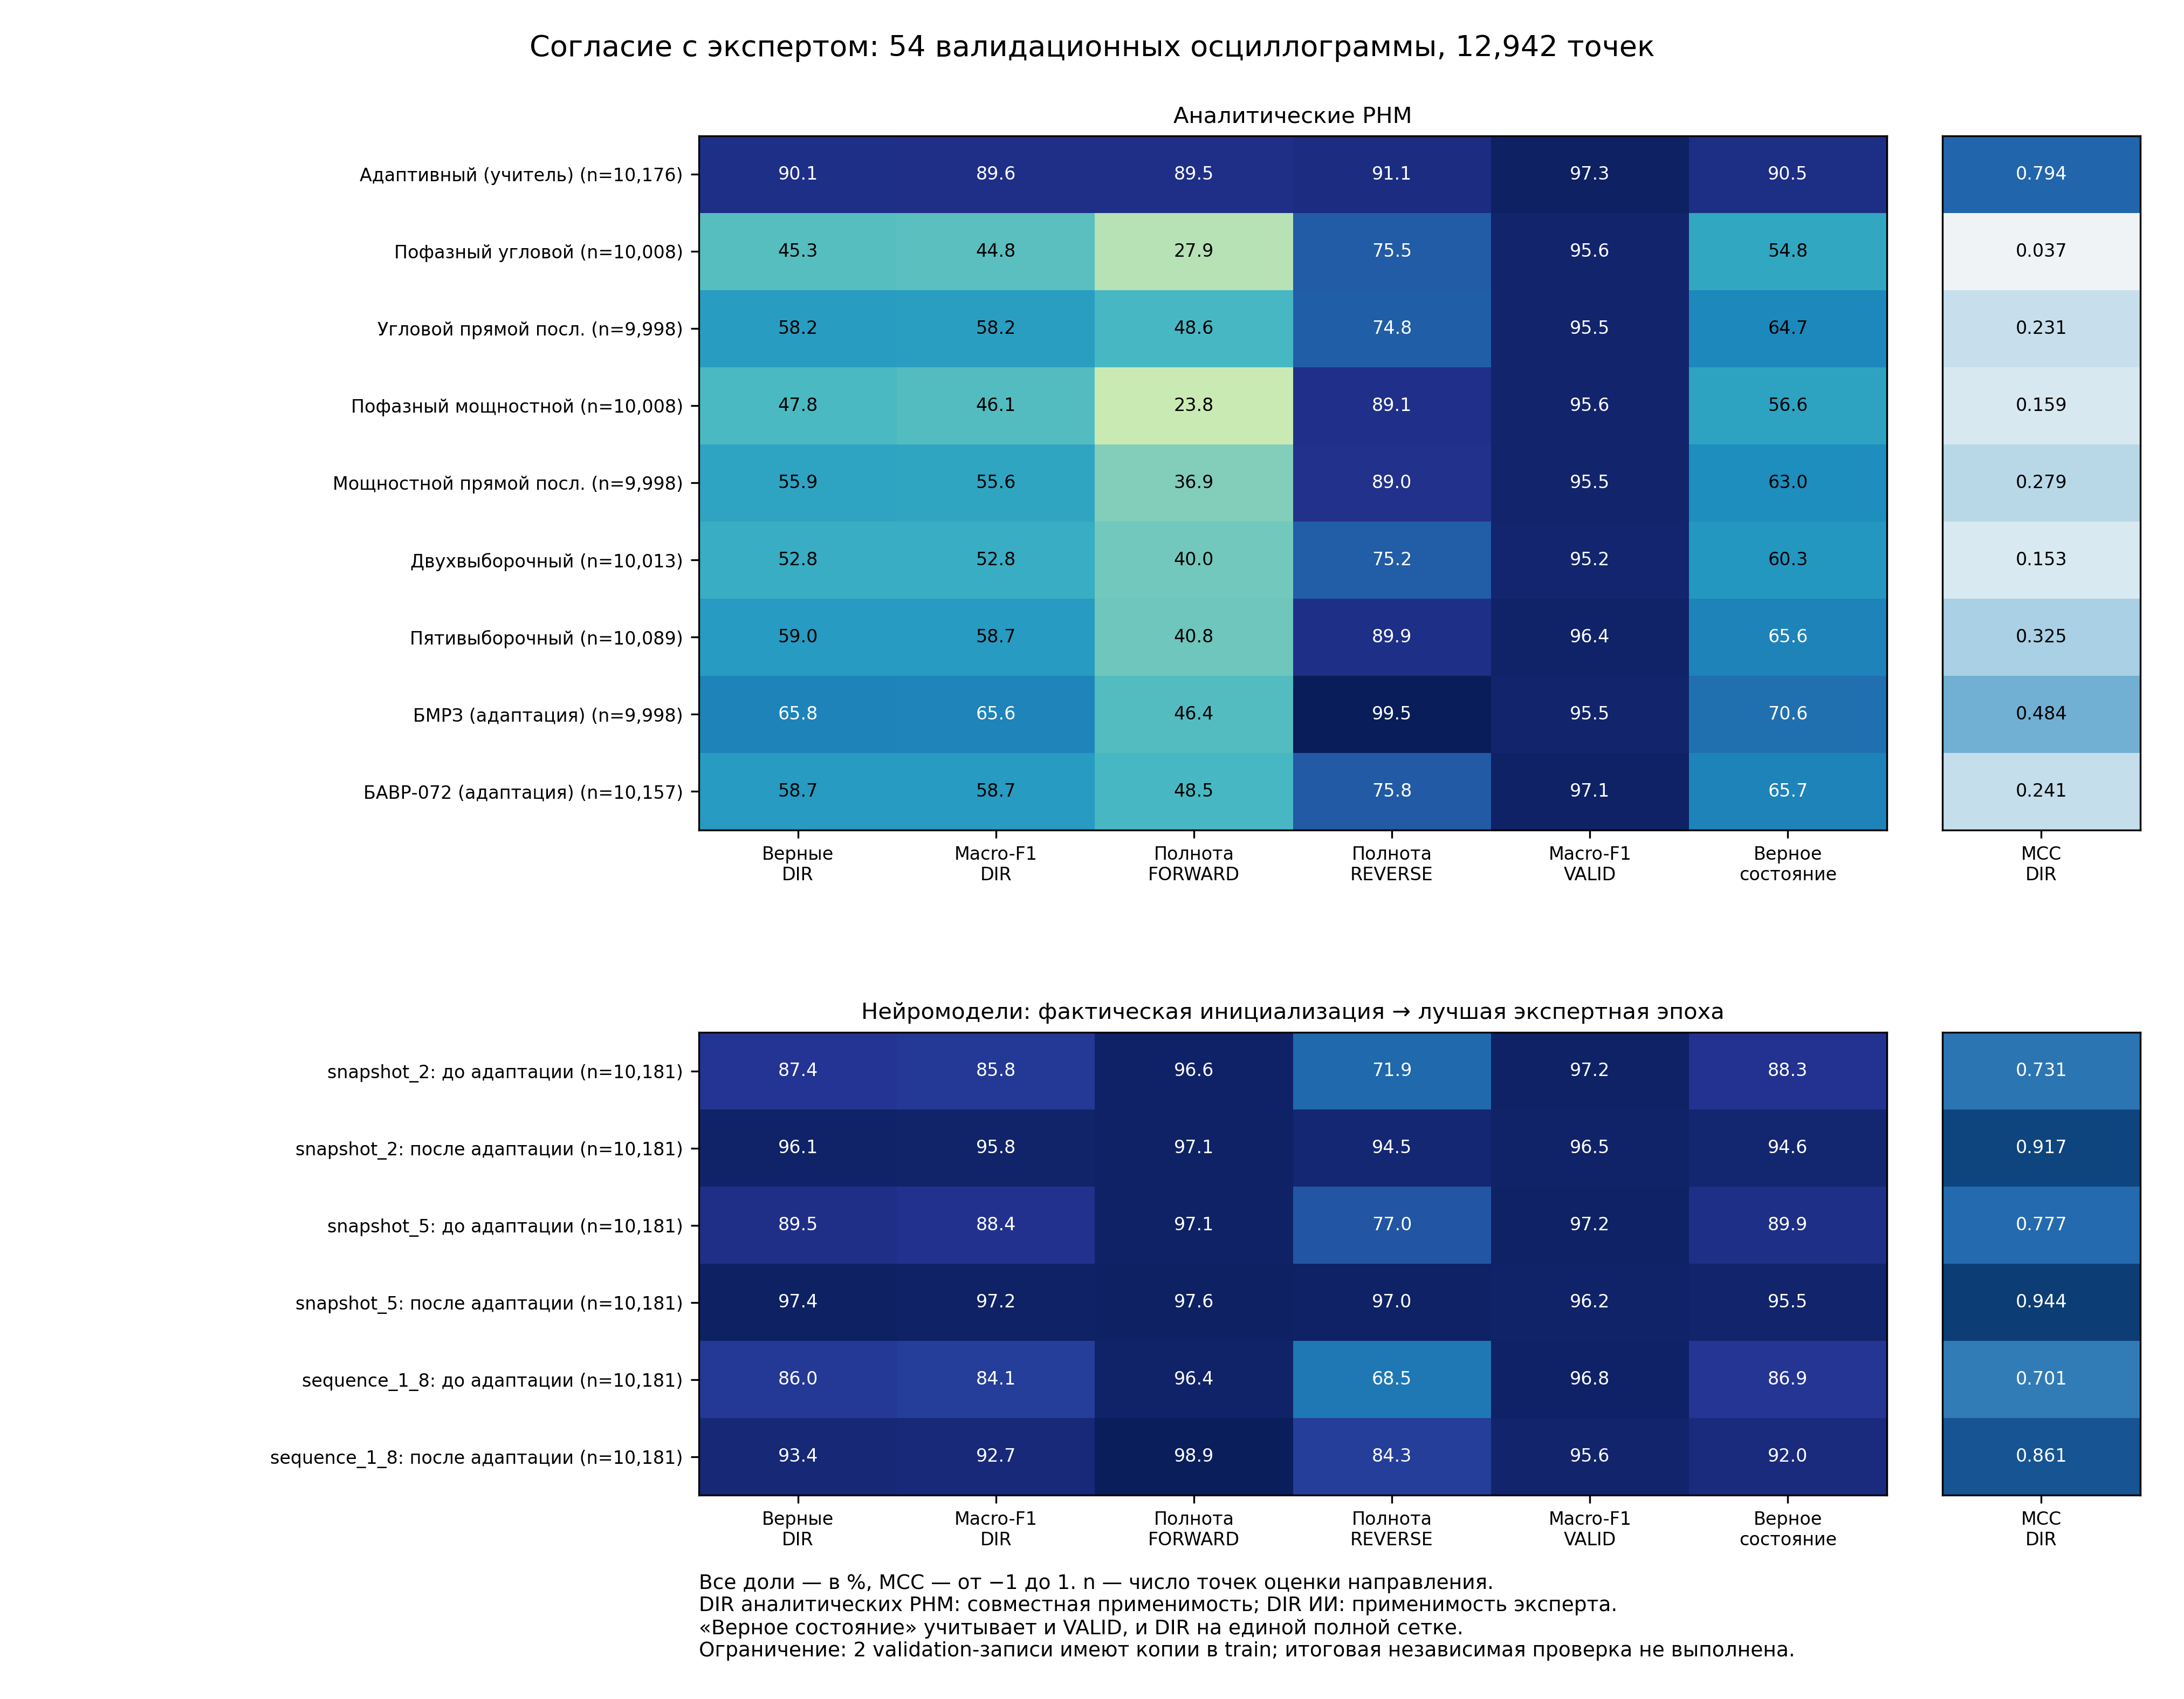
\includegraphics[width=\textwidth]{figures/ch05/ch05_expert_adaptation_comparison_article.png}
\caption{Согласие аналитических и нейросетевых органов
с экспертом. Направление оценивается на указанных
применимых точках, полное состояние на общей сетке
из 12\,942 точек 54 осциллограмм.
Процентные показатели и MCC имеют разные шкалы}
\label{fig:ch5_expert_adaptation_comparison}
\figurereview{Исходный рисунок 10 статьи 5, без перерисовки.
Для окончательного оформления увеличить мелкие подписи,
заменить snapshot/sequence русскими названиями вариантов,
сохранив числа, знаменатели и оговорку о двух копиях.}
\end{figure}

Объединённый результат также скрывает различие источников.
У модели пяти срезов Macro-F1 направления равен 95,76\%
в Open\_EE и 99,10\% во French/RTE.
Последовательная модель в Open\_EE обнаруживает
71,72\% обратных решений при 98,79\% прямых.
Для БАВР такой перекос требует отдельного разбора,
поскольку высокая полнота одного направления
не компенсирует ошибки противоположного.

Выбор промежуточного состояния существенно влияет на результат.
У модели пяти срезов последняя экспертная эпоха
имеет Macro-F1 направления 91,02\% против 97,22\%
у выбранной. Это объясняет сохранение промежуточных весов,
но одновременно сохраняет ограничение выбора по валидации.
По одному запуску каждого варианта
нельзя установить преимущество для любого объекта.

Чувствительность к составу небольшого контрольного набора
оценена повторным выбором целых исходных групп,
а не соседних отсчётов. В 54 записях выделены 53 группы
по источнику и точному совпадению входных сигналов.
Для разности Macro-F1 направления пяти и двух срезов
95\%-й интервал составляет от 0,07 до 3,36 процентного пункта,
а относительно последовательной модели
от $-0{,}35$ до 11,38 пункта.
Второй интервал включает отсутствие преимущества.
Эта проверка описывает изменение состава записей
при фиксированных весах. Случайность нового обучения
и оптимизм выбора эпохи по той же валидации
в неё не входят.

Результат показывает возможность изменить сформированное
автоматическим учителем правило с помощью экспертного материала.
Он не определяет лучшую архитектуру для всех РЗА
и не заменяет проверку длительных ошибок,
редкой неприменимости и реакций на переходы.
Более глубокая модель имеет иной спектральный состав
и другую временную сетку валидации.
Её результаты рассматриваются отдельно от этой таблицы.

\subsection{Углублённая модель с сокращённым спектральным входом}
\label{sec:ch5_h123_model}
\conceptsource{Статья 5, подраздел 9.8, таблица 12а.
Проверяется совместное изменение спектра и ёмкости модели,
а не изолированное преимущество глубины или трёх гармоник.}

Дополнительный вариант исследует другой способ
распределить сложность между входным представлением
и его нелинейной обработкой.
Сохраняются пять срезов на интервале десять периодов,
но спектр ограничивается первой, второй и третьей гармониками.
Для каждой используются модули и относительные углы
шести симметричных составляющих токов и напряжений.
Один срез содержит $6\cdot2\cdot3=36$ чисел вместо 156.

Вариант обозначен H123-D24 по трём гармоникам и 24 слоям.
Скрытая размерность увеличена до 128,
число голов внимания до восьми,
размер внутреннего нелинейного блока до 512.
Вместе с выходными головами модель содержит
5\,865\,779 обучаемых параметров.
Прежнее решение органа не подаётся на вход,
дополнительное временное подтверждение выхода не вводится.

Для Фурье теперь достаточно одного периода предыстории
перед первым срезом. Общая готовность полного входа
достигается после 11 периодов, около 220~мс при 50~Гц.
Это накопление контекста от начала записи,
а не измеренное время реакции на новое событие.
Одновременно изменены спектр, глубина и ширина сети.
Поэтому результат нельзя приписать одному из этих факторов.

Сохраняются 300 эпох предварительного и 100 эпох
экспертного обучения, ротация материала и защитная маска 5~мс.
Экспертный этап также начинается от последних предварительных весов.
Благодаря более короткой предыстории пригодны 703
экспертные обучающие записи вместо 699.
В их числе 472 записи Open\_EE и 231 French/RTE.
По совместному критерию выбраны предварительная эпоха 189
и экспертная эпоха 48.

\begin{table}[htbp]
\centering\small
\caption{H123-D24 на экспертной валидации}
\label{tab:ch5_h123_expert}
\setlength{\tabcolsep}{3pt}
\begin{tabular}{p{0.28\textwidth}rrrrr}
\toprule
Этап и веса & \shortstack{Macro-F1\\DIR, \%}
 & \shortstack{Macro-F1\\VALID, \%}
 & \shortstack{Верное\\состояние, \%}
 & \shortstack{DIR\\Open\_EE, \%}
 & \shortstack{DIR\\French/RTE, \%} \\
\midrule
Предварительные, последние & 89,46 & 97,32 & 90,15 & 83,25 & 98,66 \\
Предварительные, выбранные & 94,10 & 97,26 & 93,78 & 90,88 & 98,71 \\
Экспертные, последние & 95,99 & 96,38 & 94,68 & 95,56 & 96,56 \\
Экспертные, выбранные & 97,33 & 97,20 & 96,23 & 95,84 & 99,40 \\
\bottomrule
\end{tabular}
\end{table}

В таблице~\ref{tab:ch5_h123_expert} DIR обозначает направление,
VALID применимость. Сетка включает 54 записи,
13\,223 точки применимости и 10\,506 точек направления.
Относительно фактической инициализации Macro-F1 направления
вырастает на 6,53 пункта для последних экспертных весов
и на 7,87 для выбранных.
Однако после выбранной эпохи ухудшаются
и направление, и полное состояние.

Список файлов совпадает с компактным сравнением,
но более короткая предыстория изменяет допустимые точки.
В новой сетке на 281 точку применимости
и на 325 точек направления больше.
Разность 97,33 и 97,22\% поэтому
не доказывает преимущества углублённой модели.
Для временного сопоставления далее используется
общая плотная сетка и одинаково выбранный тип весов.

\iffalse
(Примечание автора: НУ и какие выводы об этой модели в сравнении с другими? Может её потом вообще выкину..)
\fi
\authorreviewnote{AA187}

\subsection{Динамика обучения и сохранение прежних режимов}
\label{sec:ch5_training_dynamics}
\conceptsource{Статья 5, рисунок 9, таблица 12б и рисунок 10а.
Отдельно мониторинг по эпохам и полное пофайловое прохождение
автоматической validation-части.}

Динамика обеих стадий приведена на
рисунках~\ref{fig:ch5_training_dynamics_snapshots}
и~\ref{fig:ch5_training_dynamics_sequence}.
Сверху показано согласие с автоматическим учителем,
снизу с экспертным решением.
Разность между верхней и нижней кривыми
не является приростом одной метрики на одном наборе.
Четвёртая конфигурация имеет отдельную временную сетку.
Отмеченная эпоха выбрана по совместному критерию двух выходов,
а не обязательно по максимуму изображённого Macro-F1.

\begin{figure}[p]
\centering
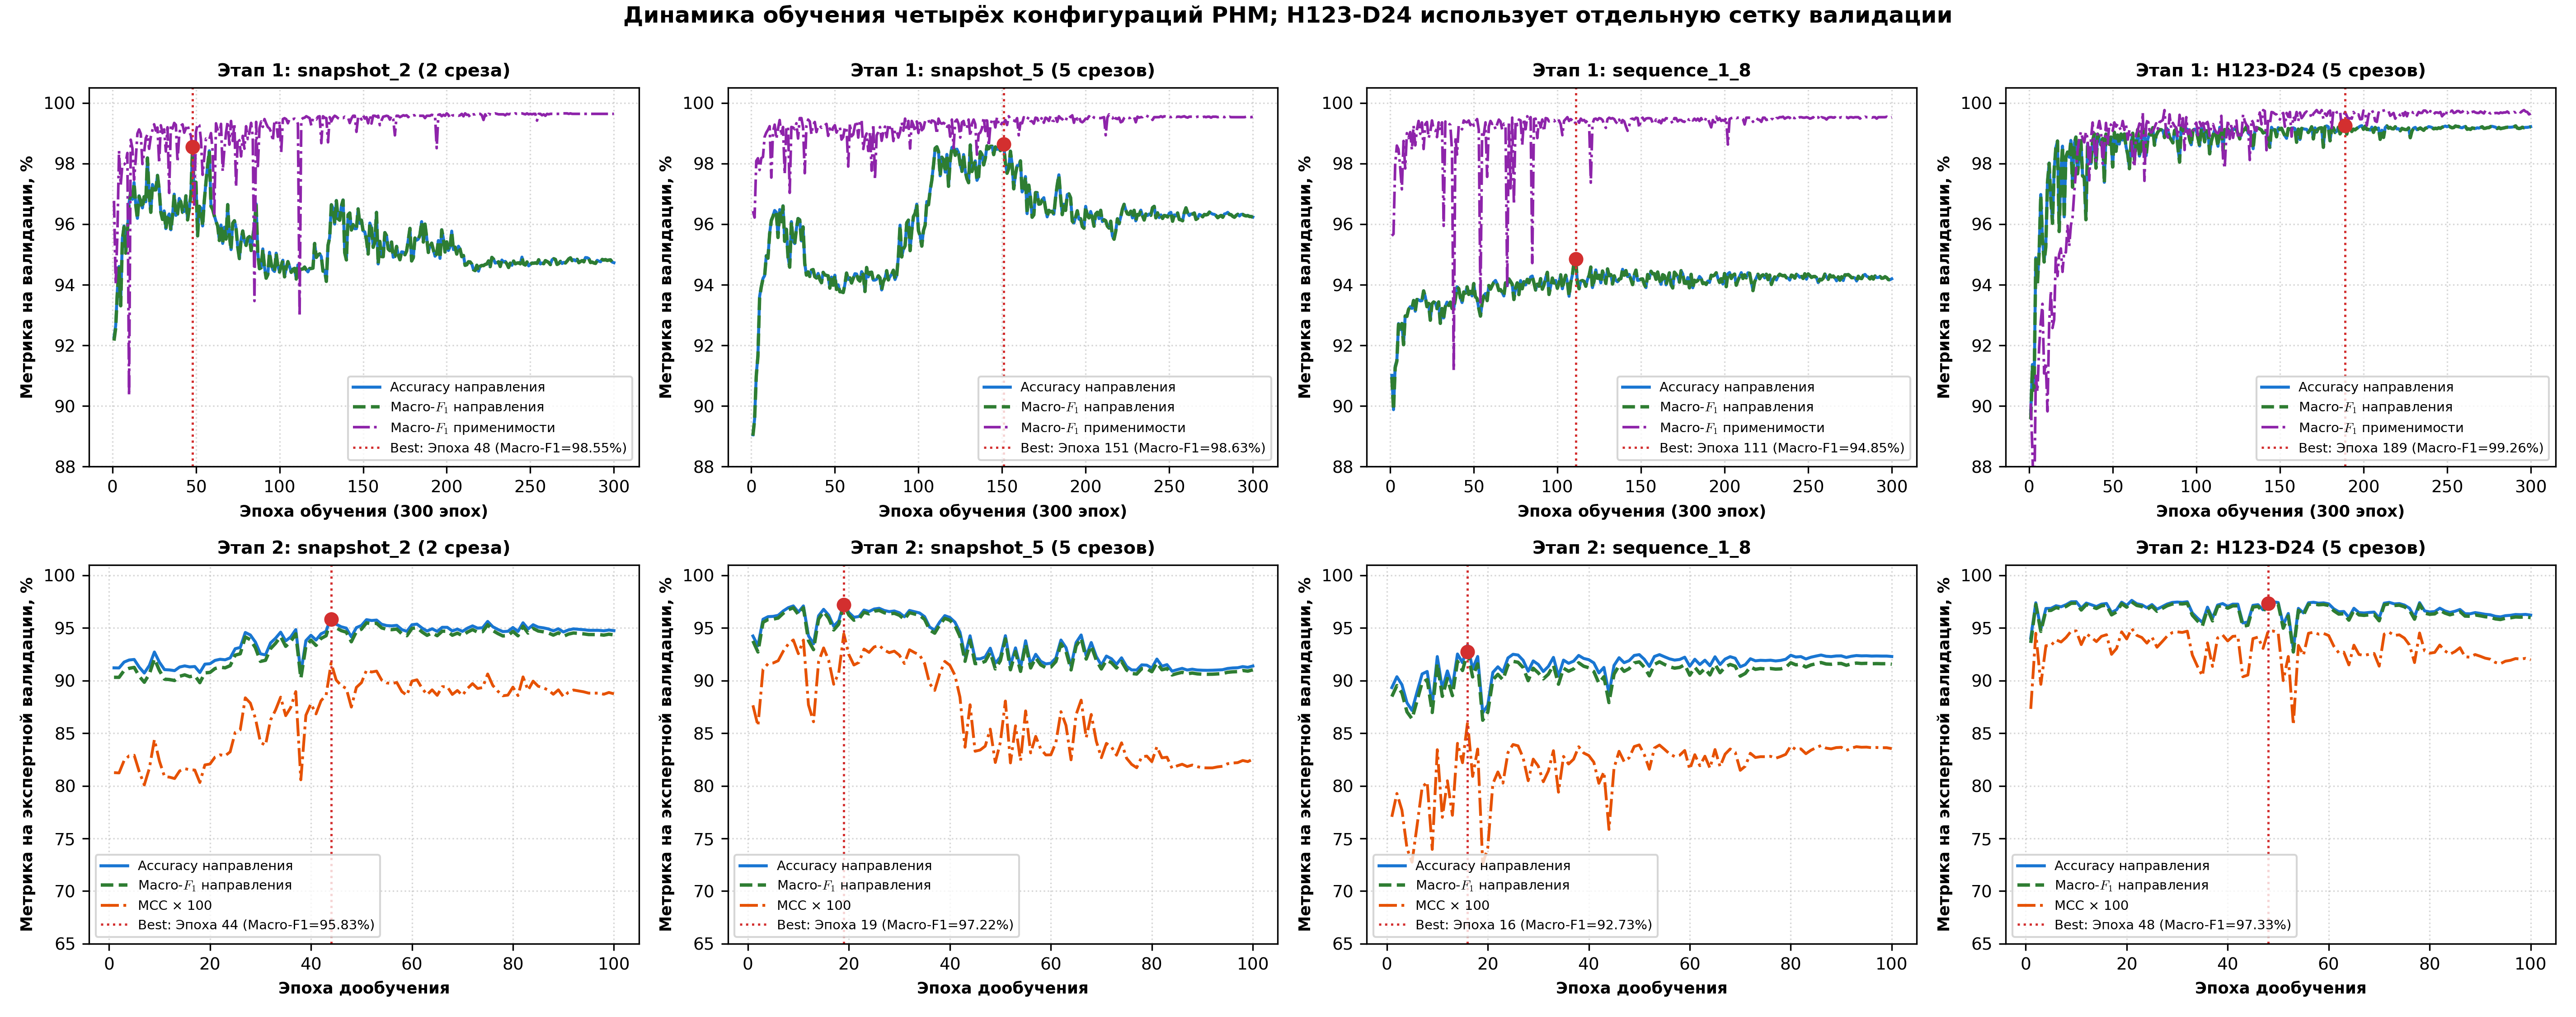
\includegraphics[width=\textwidth,trim=0bp 0bp 684bp 21.6bp,clip]{figures/ch05/ch05_training_dynamics_article.png}
\caption{Динамика предварительного и экспертного обучения
моделей с двумя и пятью срезами.
Верхний ряд относится к автоматическому учителю,
нижний к эксперту}
\label{fig:ch5_training_dynamics_snapshots}
\figurereview{Левая половина исходного рисунка 9 статьи 5.
Изображение разделено средствами вёрстки, кривые не перестроены.
Заменить Accuracy и Best русскими подписями.
Отметка выбранной эпохи не является максимумом каждой кривой.}
\end{figure}

\begin{figure}[p]
\centering
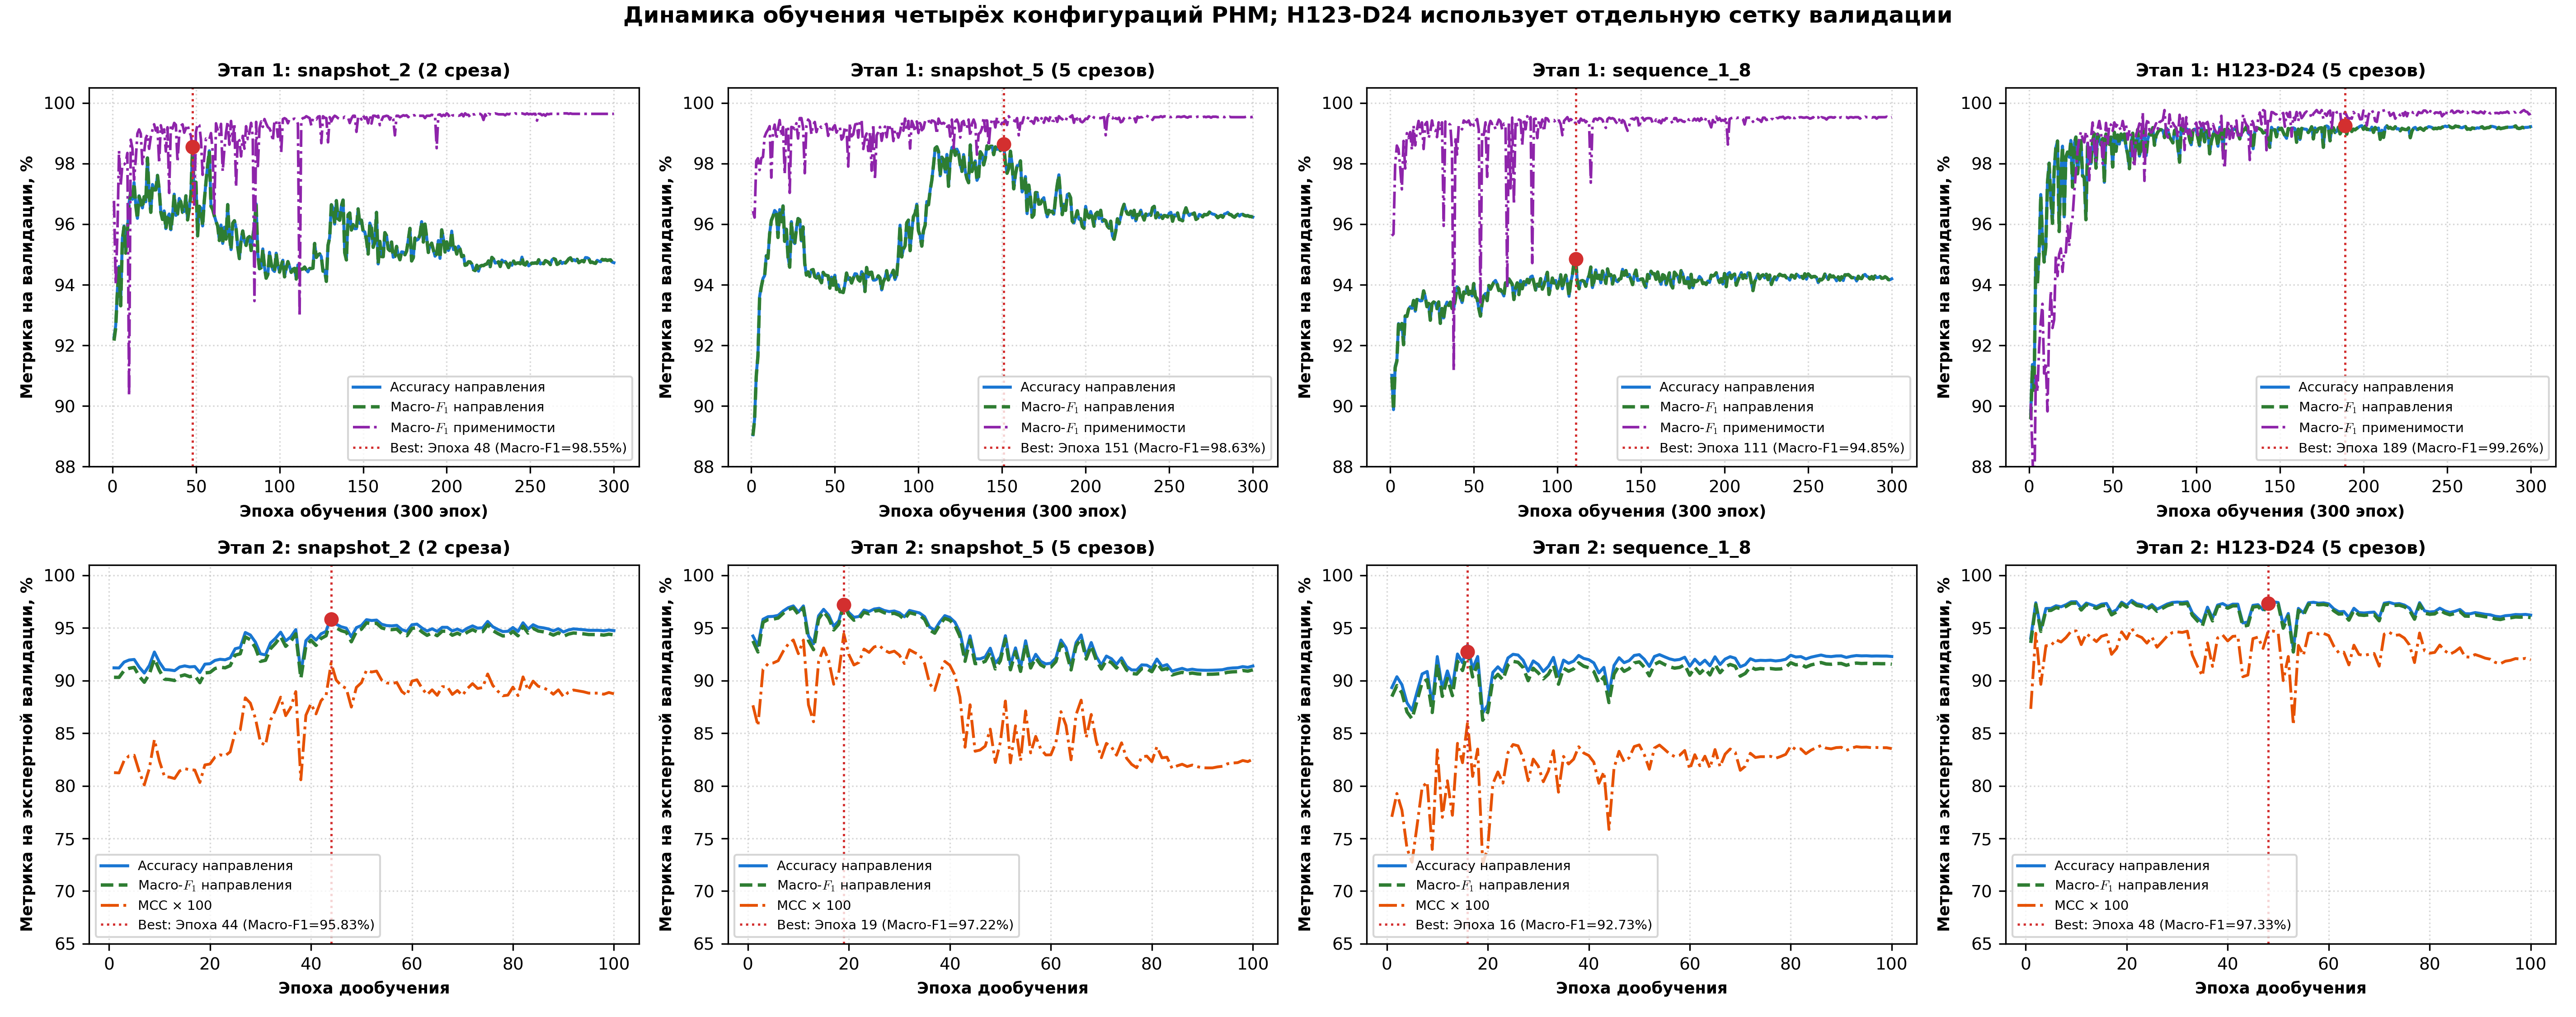
\includegraphics[width=\textwidth,trim=684bp 0bp 0bp 21.6bp,clip]{figures/ch05/ch05_training_dynamics_article.png}
\caption{Динамика обучения последовательной модели и H123-D24.
Верхний и нижний ряды используют разные эталоны,
H123-D24 также имеет отдельную сетку валидации}
\label{fig:ch5_training_dynamics_sequence}
\figurereview{Правая половина исходного рисунка 9 статьи 5.
Верхняя панель H123-D24 показывает мониторинговую часть,
а не полное пофайловое прохождение из следующего сравнения.
Не заменять одно число другим без различения этих наборов.
Перевести Accuracy и Best, сохранив значения и выбранные эпохи.}
\end{figure}

Для H123-D24 дополнительно пройдена вся автоматическая
валидационная часть из 3028 исходных идентификаторов.
Допустимые цели имеются в 2603 записях,
остальные 425 их не образуют при принятом входном контракте.
Из каждой пригодной записи проверяется до 32 точек.
Всего получены 83\,296 точек применимости
и 76\,693 точки направления.
Это полное прохождение списка файлов,
но не проверка каждого отсчёта записи.

Результат на двух эталонах показан на
рисунке~\ref{fig:ch5_h123_references}.
На автоматическом материале Macro-F1 направления
последних весов снижается с 98,57\% перед экспертным этапом
до 96,92\% после него.
Во French/RTE снижение равно 2,96 пункта,
в Open\_EE 0,51 пункта.
Одновременно согласие с экспертом возрастает.

\begin{figure}[htbp]
\centering
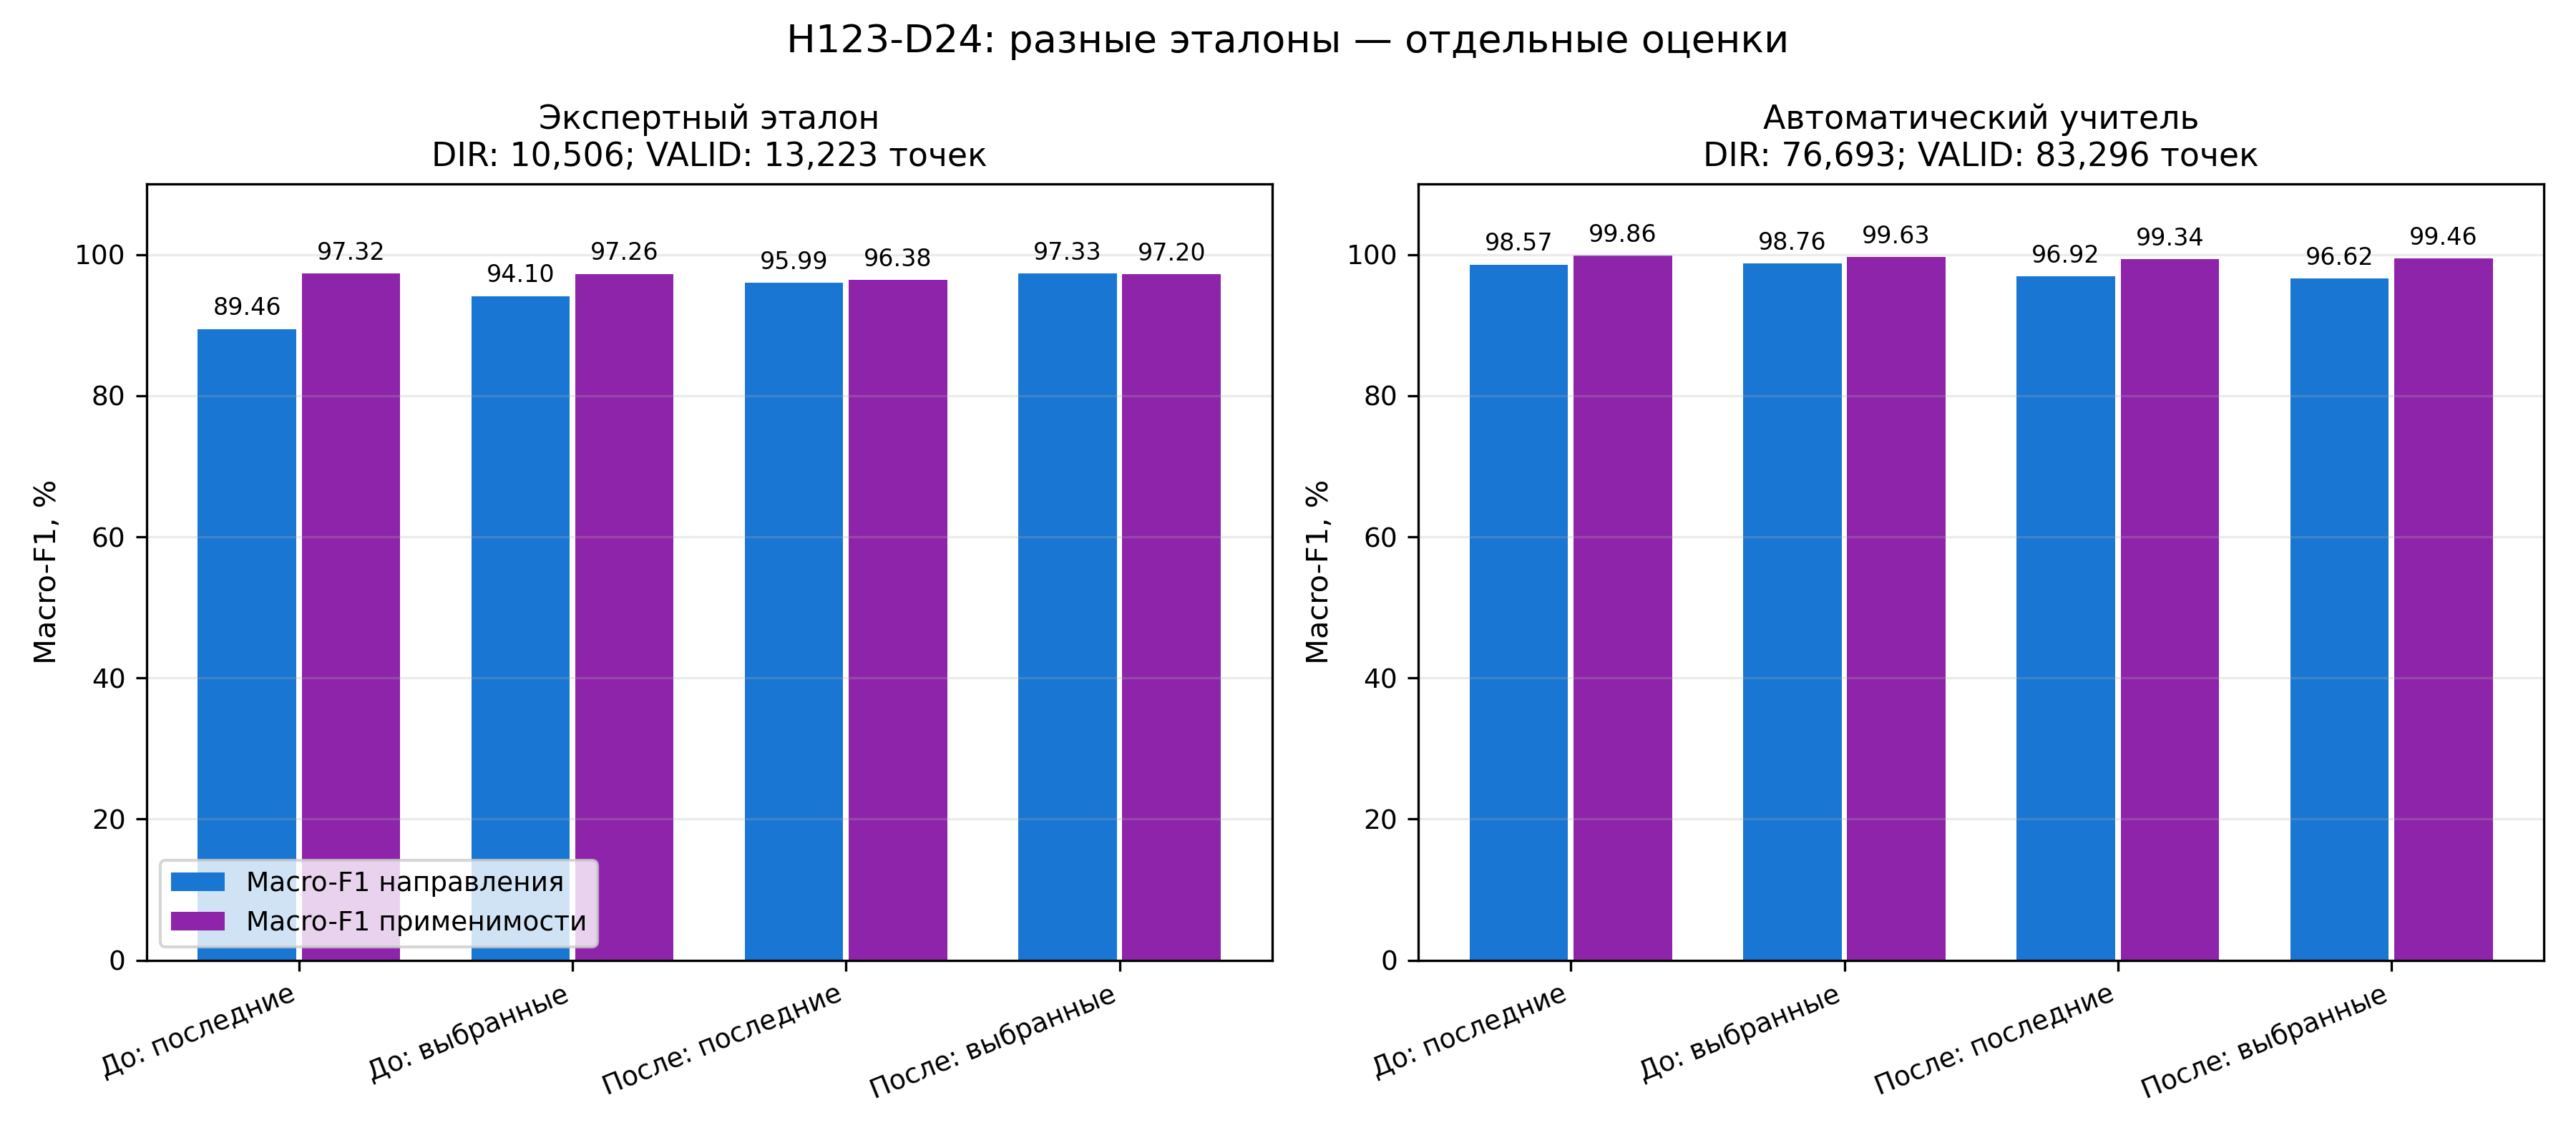
\includegraphics[width=\textwidth]{figures/ch05/ch05_h123_evaluation_article.png}
\caption{Отдельная оценка H123-D24 по экспертному эталону
и автоматическому учителю.
Внутри панели сохранена общая сетка,
между панелями различаются данные и эталон}
\label{fig:ch5_h123_references}
\end{figure}
\figurereview{Исходный рисунок 10а статьи 5.
Заменить DIR и VALID понятными русскими обозначениями,
«До» и «После» уточнить как до и после экспертного этапа.
Столбцы между панелями не показывают прирост качества.}

Снижение согласия с учителем может означать
как полезное исправление его ограничений,
так и потерю части прежнего поведения.
Само по себе оно не различает эти причины.
Поэтому наличие буфера обычных режимов
не принимается за доказательство отсутствия забывания.
Плотная экспертная и дополнительная режимная проверка
нужны независимо от того, какой эталон
даёт модели более высокую среднюю оценку.


\subsection{Поведение органов на отдельных осциллограммах}
\label{sec:ch5_waveform_cases}
\textcolor{red}{В работе. Физическое описание случаев и окончательные
рисунки ещё не подготовлены для вычитки.}

Для оценки РНМ нужно видеть токи и напряжения вместе с ответами
органов на одной временной оси. На такой записи можно различить
ошибочное направление, колебания выхода и отсутствие пригодного
ответа. Эти особенности могут скрываться за близкими сводными оценками.
В статье для этого предусмотрены шесть панелей рисунка 11.
Ниже закреплены места для их авторской доработки.
Названия процессов из демонстрационной версии пока не принимаются
за завершённую физическую классификацию.

\begin{figure}[htbp]
\centering
\fbox{\begin{minipage}{0.92\textwidth}
\centering\textbf{Место для осциллограммы 1}\par\medskip
Три фазных тока и напряжения на общей временной шкале.\par
Ниже состояния аналитических органов, модели и экспертная разметка.\par
Отдельно показать неприменимые интервалы и границу перехода.
\end{minipage}}
\caption{Пример 1 совместного рассмотрения измерений и выходов РНМ.
Панель рисунка 11 статьи подлежит авторской доработке}
\label{fig:ch5_waveform_case_1}
\end{figure}

\begin{figure}[htbp]
\centering
\fbox{\begin{minipage}{0.92\textwidth}
\centering\textbf{Место для осциллограммы 2}\par\medskip
Три фазных тока и напряжения на общей временной шкале.\par
Ниже состояния аналитических органов, модели и экспертная разметка.\par
Отдельно показать неприменимые интервалы и границу перехода.
\end{minipage}}
\caption{Пример 2 совместного рассмотрения измерений и выходов РНМ.
Панель рисунка 11 статьи подлежит авторской доработке}
\label{fig:ch5_waveform_case_2}
\end{figure}

\begin{figure}[htbp]
\centering
\fbox{\begin{minipage}{0.92\textwidth}
\centering\textbf{Место для осциллограммы 3}\par\medskip
Три фазных тока и напряжения на общей временной шкале.\par
Ниже состояния аналитических органов, модели и экспертная разметка.\par
Отдельно показать неприменимые интервалы и границу перехода.
\end{minipage}}
\caption{Пример 3 совместного рассмотрения измерений и выходов РНМ.
Панель рисунка 11 статьи подлежит авторской доработке}
\label{fig:ch5_waveform_case_3}
\end{figure}

\begin{figure}[htbp]
\centering
\fbox{\begin{minipage}{0.92\textwidth}
\centering\textbf{Место для осциллограммы 4}\par\medskip
Три фазных тока и напряжения на общей временной шкале.\par
Ниже состояния аналитических органов, модели и экспертная разметка.\par
Отдельно показать неприменимые интервалы и границу перехода.
\end{minipage}}
\caption{Пример 4 совместного рассмотрения измерений и выходов РНМ.
Панель рисунка 11 статьи подлежит авторской доработке}
\label{fig:ch5_waveform_case_4}
\end{figure}

\begin{figure}[htbp]
\centering
\fbox{\begin{minipage}{0.92\textwidth}
\centering\textbf{Место для осциллограммы 5}\par\medskip
Три фазных тока и напряжения на общей временной шкале.\par
Ниже состояния аналитических органов, модели и экспертная разметка.\par
Отдельно показать неприменимые интервалы и границу перехода.
\end{minipage}}
\caption{Пример 5 совместного рассмотрения измерений и выходов РНМ.
Панель рисунка 11 статьи подлежит авторской доработке}
\label{fig:ch5_waveform_case_5}
\end{figure}

\begin{figure}[htbp]
\centering
\fbox{\begin{minipage}{0.92\textwidth}
\centering\textbf{Место для осциллограммы 6}\par\medskip
Три фазных тока и напряжения на общей временной шкале.\par
Ниже состояния аналитических органов, модели и экспертная разметка.\par
Отдельно показать неприменимые интервалы и границу перехода.
\end{minipage}}
\caption{Пример 6 совместного рассмотрения измерений и выходов РНМ.
Панель рисунка 11 статьи подлежит авторской доработке}
\label{fig:ch5_waveform_case_6}
\end{figure}
